
\section{Spatial Verification Results}

Our initial results on the Todai dataset were not surprising.  The diurnal pattern dominates the comparison between the sensors.
Weather is the main driver for this behavior and it affects the readings in almost all of the
sensors in our dataset.  Cross-correlation on raw sensor data is insufficient for filtering intrinsically related
behavior.  Upon closer examination of the data we assess the following:

\begin{itemize}
\item The main underlying diurnal trend occurs in almost all the traces.
\item Occupancy and room activities occur at random times during the day and change 
		at a higher frequency than weather patterns.
\item Sensors that serve the same location observe the same activities.  Therefore, their underlying
		measurements should be correlated.
\end{itemize}

In order to uncover these relationships we must remove low-frequency trends in the traces and
compare the readings at high frequencies.

\begin{table}
\begin{center}
\begin{tabular}{|l|l|l|l|l|l|}
\hline
 & Raw trace & 1st IMF & 2nd IMF & 3rd IMF & Residual\\ \hline
EHP, Light & 0.7715 & 0.43909 & 0.49344 & 0.63469 & 0.82132 \\ \hline
EHP, GHP & 0.6370 & 0.0060274 & 0.063546 & 0.16764 & 0.79378 \\ \hline
\end{tabular}
\caption{Correlation coefficients of the analyzed trace and their IMFs uncovered by EMD}
\label{tab:corr}
\end{center}
\end{table}


% \subsection{Simple Scenario}
We test our hypothesis in this section by using EMD to remove low-frequency trends in the data
and run correlation calculation at overlapping IMF timescales.  We discover that EMD allows us
to find and compare high-frequency instrinsic behavior that is spatially correlated across
sensors.  We begin with a small set of three sensors (EHP, GHP, light) and expand our scope
to include all the sensors in the dataset.







\subsection{Initial Todai Analysis Results}


\begin{figure}[th!]
\hspace{-2cm}
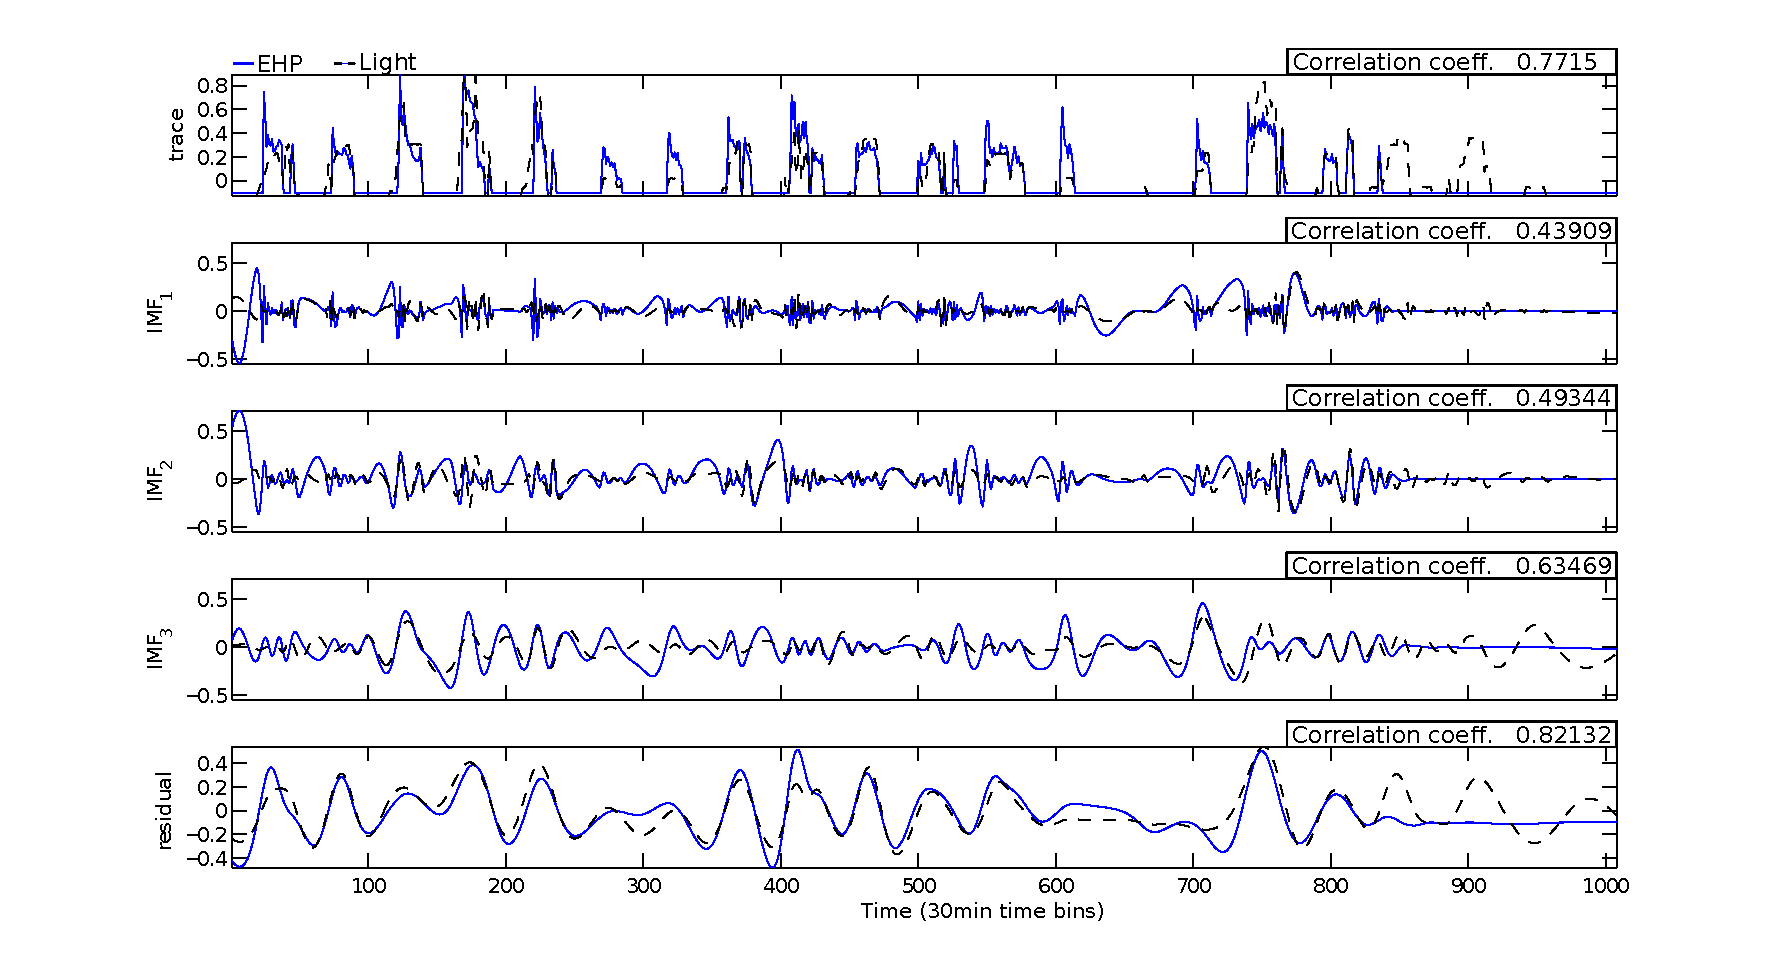
\includegraphics[width=1.2\textwidth]{figs/emd_25_26-eps-converted-to}
\vspace{-1cm}
\caption{Decomposition of the EHP and light trace using bivariate EMD. IMFs correlation coefficients highlight the intrinsic relationship of the two traces.}
\label{fig:emd}
\end{figure}

Figure~\ref{fig:emd} shows the raw traces for the three devices discussed in 
the previous section (EHP, GHP, light). All three exhibit a diurnal usage pattern.  On weekends, each
draw less power.   For our initial analysis, we calculated the pairwise 
correlation coefficient for all sensors in the set.  The correlation coefficient for 
 the EHP and light is $0.7715$ and the correlation coefficient for the EHP and GHP is $0.6370$.
Running correlation across them yields high correlation coefficients, mostly
due to their underlying daily usage pattern.

% Lets consider the simple example of Section \ref{problem} where 
We would like to know if the EHP trace is correlated with the two other traces.
Recall that the correlation coefficients of the raw feeds was $0.7715$ and $0.6370$, corresponding to the light 
and GHP, respectively.
As stated in previous section this result is correct but not so meaningful, since most of the traces
display the same diurnal pattern.
Figure \ref{fig:emd} and Figure \ref{fig:emd2} show the EMD decomposition of the three traces.
For each trace, EMD has retrieved three IMFs that highlight the higher frequencies of the traces.

Figure~\ref{fig:emd} shows the normalized raw trace (top) and EMD output IMFs and residual as well as the 
correlation coefficients calculated on the IMFs for the EHP and
light traces.  The correlation coefficients are $0.43909$, $0.49344$ and $0.63469$ corresponding to the IMF1, 
IMF2, and IMF3, respectively.  Notice the high correlation between the high-frequency IMFs.
We know that the light and EHP serve the same room, and their high-frequency IMF correlation corroborates
our prior knowledge.
Figure~\ref{fig:emd2} shows a complementary result, for the EHP and GHP comparison.
The correlation coefficients for the EHP and GHP IMFs suggest that the two may be independent.  In fact, they
\emph{are} indepdent; they serve completely different rooms in the building.
EMD allows us to remove low-frequency trends that add noise to the original analysis.
By comparing IMFs, we see both intrisically correlated and \emph{uncorrelated} behavior.  
% In the next
% section we expand our analysis and show the effectiveness of our methodology. 
% Although promising, these results must be validated across the rest of the
% dataset to confirm their significance.  







\subsubsection{Initial Observations}
% To validate the effectiveness of our approach, 
We analyze the same three-week time span for \emph{all} 674 sensors deployed at Todai.
For each trace $S$ we compute two scores: (1) the correlation coefficient between $S$ and the EHP trace
and (2) the average value of the IMF correlation coefficients.

\begin{figure}[tbh!]
\centering
 \subfloat[Raw traces correlation coefficients]{\label{fig:histo1}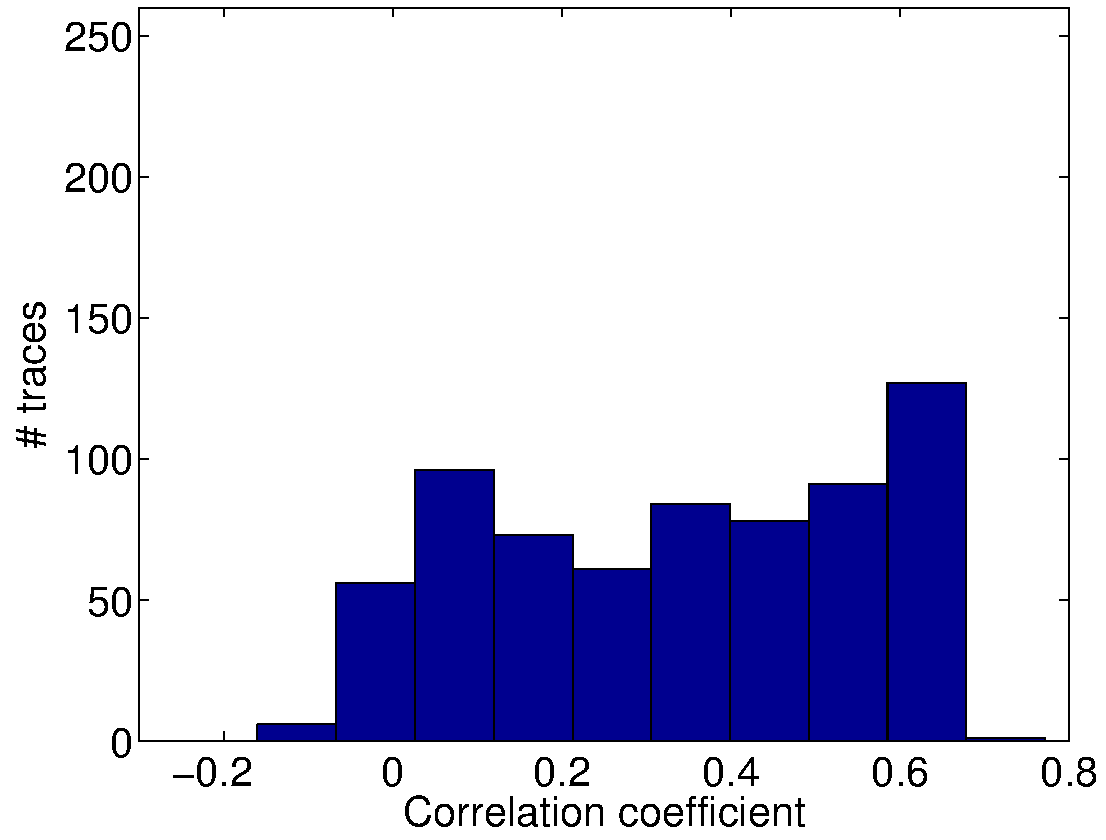
\includegraphics[width=.43\textwidth]{figs/allFloors_week1_week4_corr_abs-eps-converted-to}}
 \subfloat[Average IMFs correlation coefficients]{\label{fig:histo2}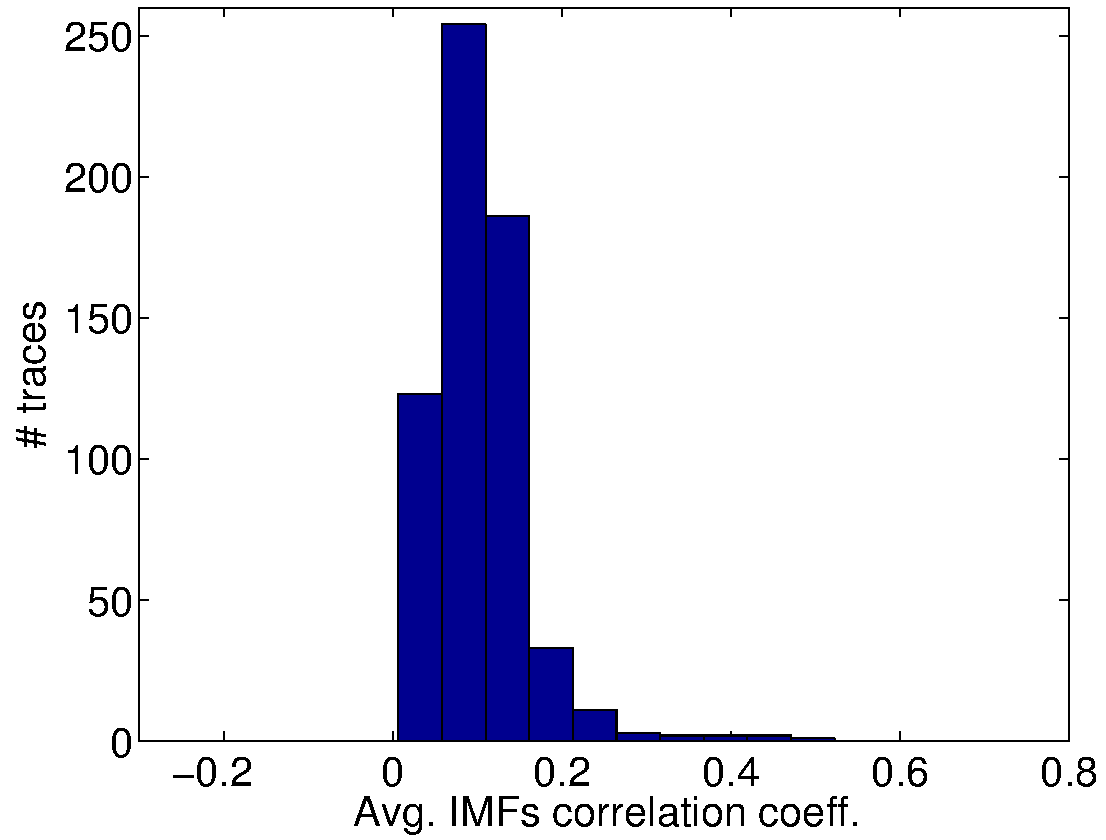
\includegraphics[width=.43\textwidth]{figs/allFloors_week1_week4_emd_abs-eps-converted-to}}
 \caption{Distribution of the correlation coefficients of the raw traces and correlation coefficients average of the corresponding IMFs using 3 weeks of data from 674 sensors.}
\label{fig:histo}
\end{figure}

\begin{figure}
\centering
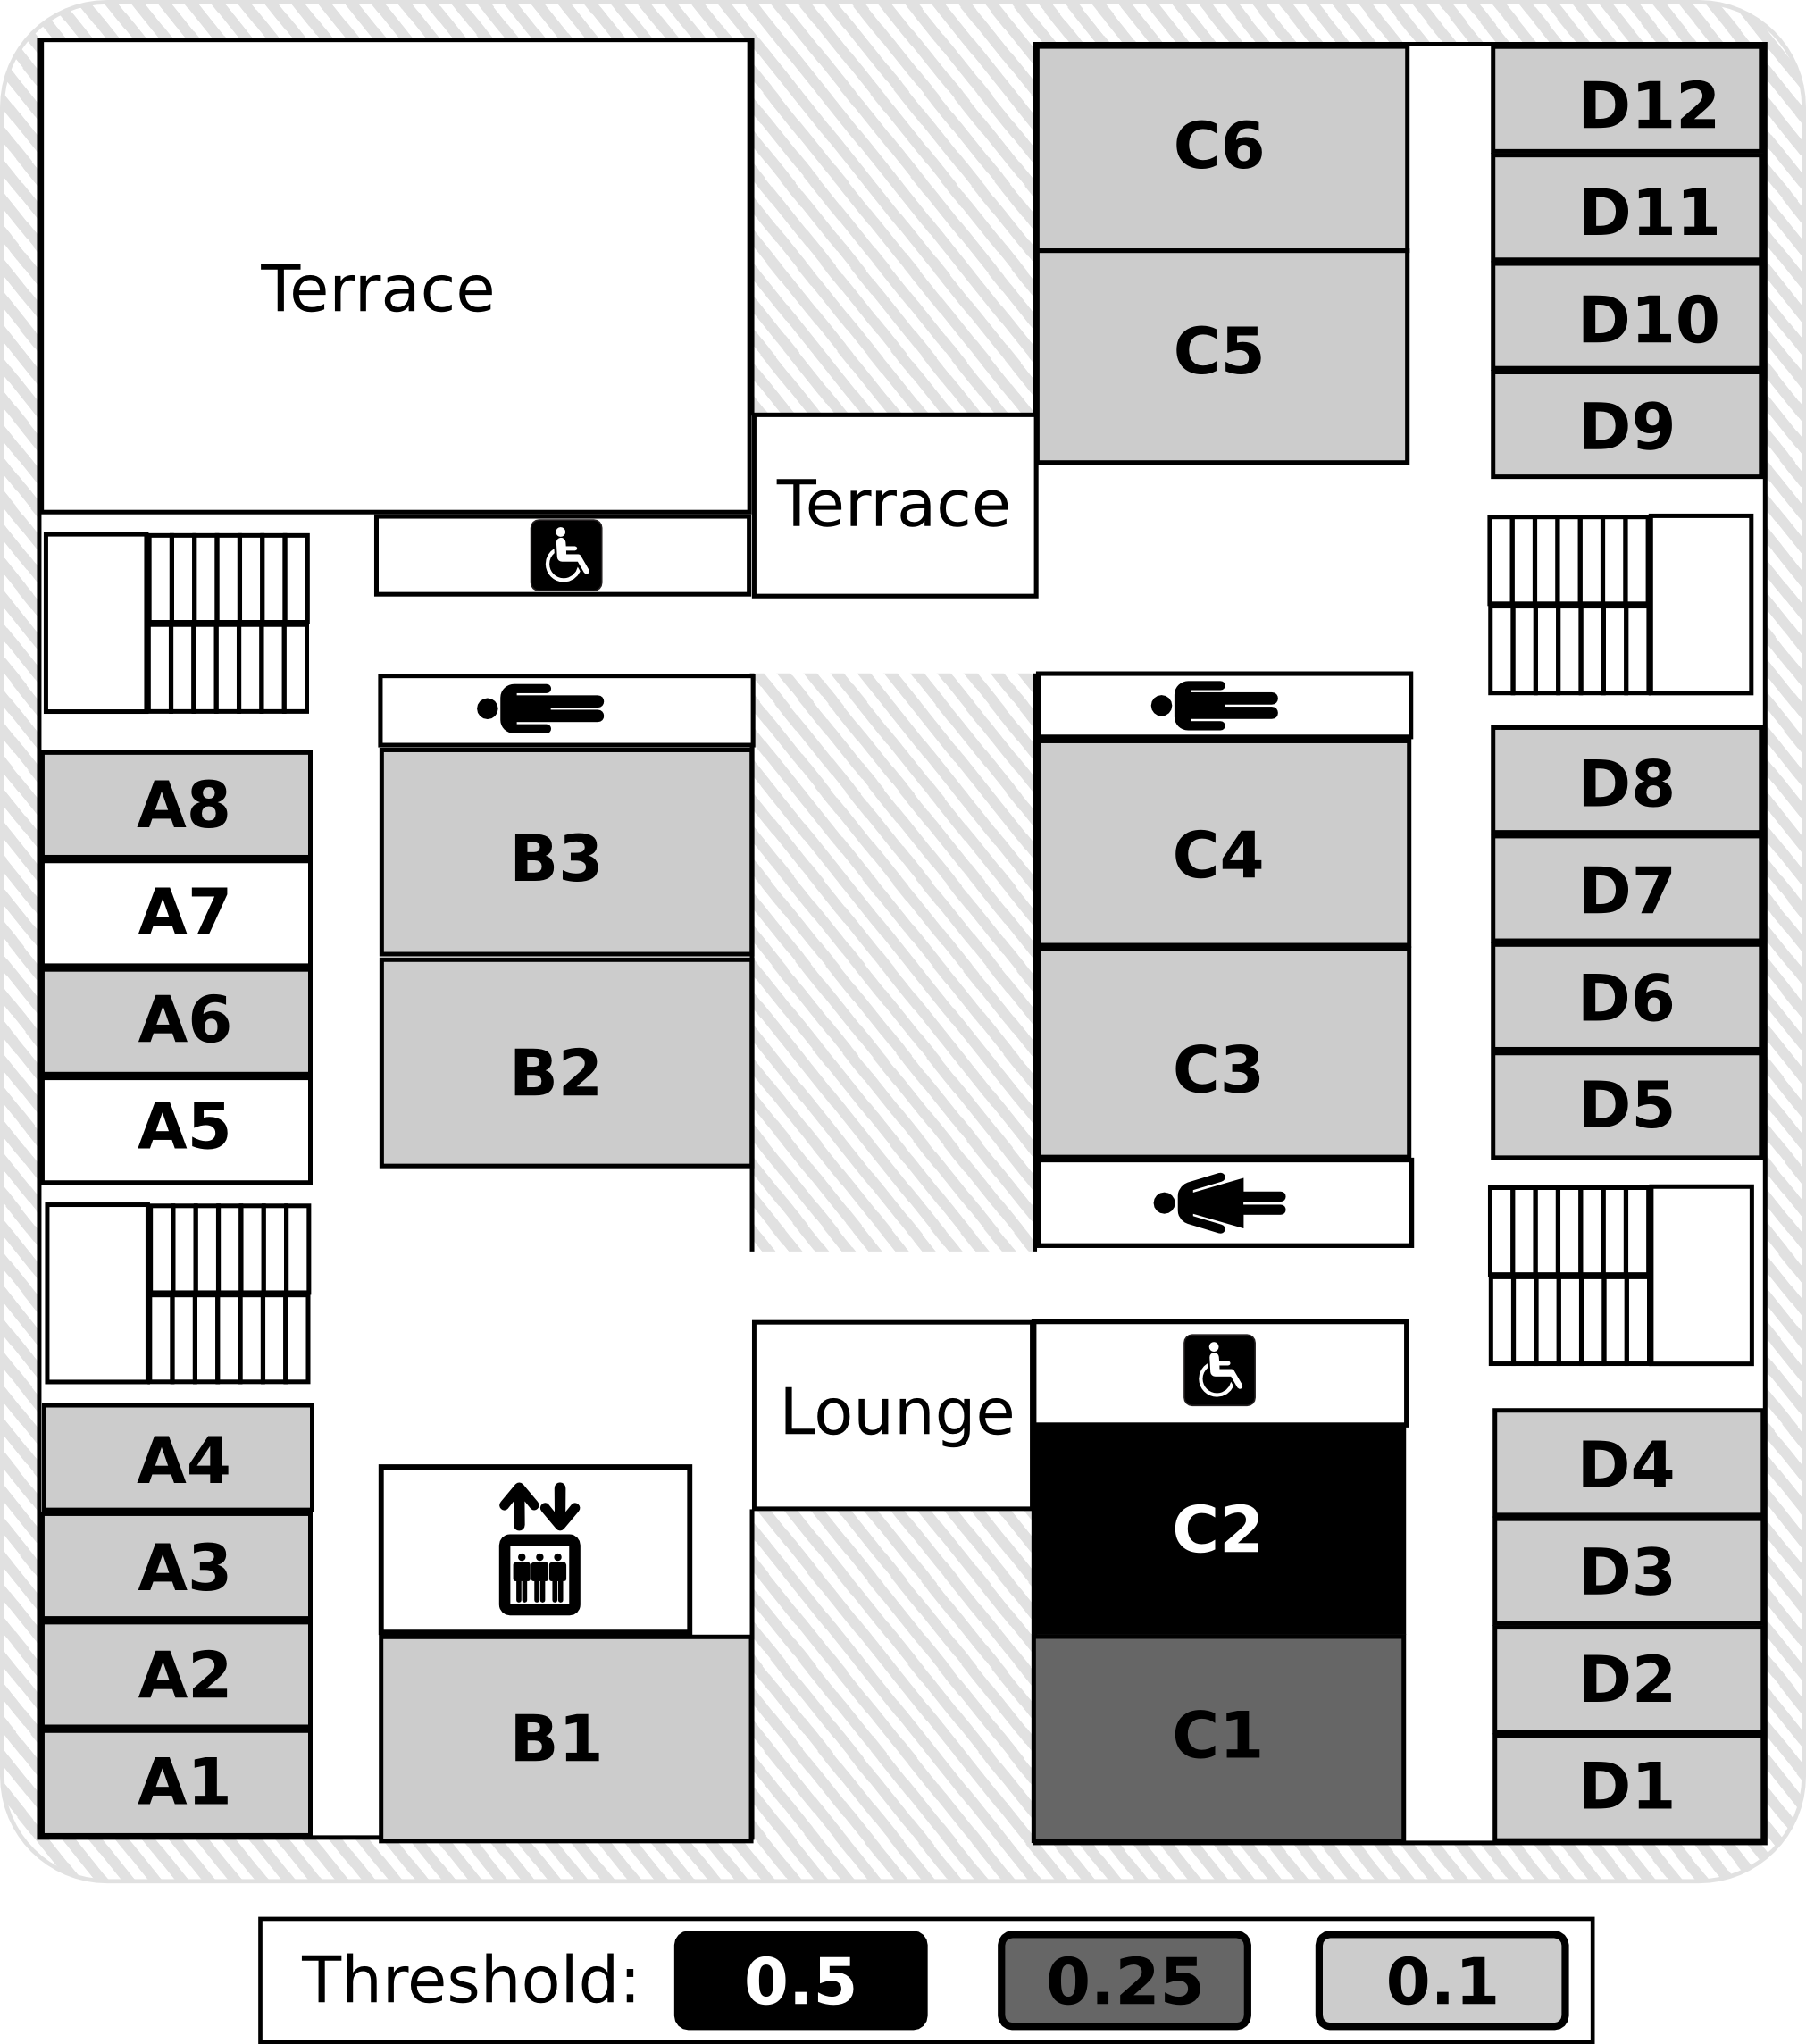
\includegraphics[width=.45\textwidth]{figs/floorMap.png}
\caption{Map of the floor where the analyzed EHP serves (room $C2$). The location of the sensors identified as related by the proposed approach are highlighted, showing a direct relationship between IMF correlation and spatial proximity.}
\label{fig:map}
\end{figure}

Figure \ref{fig:histo1} shows the distribution correlation coefficients.  Notice
that a large fraction of the dataset is correlated with the EHP trace.
\emph{Half} the traces have a correlation coefficient higher than $0.36$.  As expected, the underlying
trend is shared by a large number of device.
Although the highest score (i.e. $0.7715$) corresponds to the light in the same room that the EHP serves,
there are 118 pumps, serving all areas of the building, with a correlation higher than $0.6$.
Using only these results, it is not clear where the threshold should be set.  The distribution is close to 
uniform, making it difficult to 
know of how well your threshold discriminates against unrelated traces.
% Moreover, the distribution of the traces is almost uniform, thus, discriminating correlated traces is a laborious task.

Figure \ref{fig:histo2} shows the distribution of the average correlation value for the IMFs of
each trace and the EHP.  The number of traces correlated in the high frequency IMFs is significantly smaller
than the previous results. It's clear from the distribution that only a small set of devices are
\emph{intrinsically correlated} with the EHP.  In fact, \emph{only 10 traces out of 674} yielded a score higher than 
$0.25$. This allows us to easily rank traces by correlation.

Upon closer inspection of the 10 most correlated IMF traces, we find that there is a spatial relationship
between the EHP and the ten devices.  In fact, there is a direct relationship between score and distance from
the areas served by the EHP.  Figure~\ref{fig:map} shows a map of the floor that contains the rooms served by this
EHP.  The EHP directly serves room $C2$.  We introduce a correlation threshold to cluster correlated traces by score.
We highlight rooms by the threshold setting on the IMF correlation score.
When we set the threshold at $0.5$ we see that the sensors that have a correlation higher fall within room $C2$ --
the room served directly by the EHP.  As we relax the threshold, lowering it to $0.25$ and $0.1$ we see radial expansion from $C2$.  The trace with the highest score, $0.522$, is the trace corresponding to the lighting system \emph{in
the same room}.
The two highest scores for this floor (i.e. $0.316$ and $0.279$) are the light and EHP traces from next door, room $C1$.
Lower values correspond to sensors measuring activities in other rooms that have no specific relationship to the analyzed trace.  The results show a direct relationship between IMF correlation and spatial proximity and \emph{supports our initial
hypothesis}.

EMD is useful for finding underlying behavioral relationships between traces of sensor data.  However,
when we set the timescales smaller than a day, the results were not as strong.
The trace has to be long enough to capture the trend.  For this data set, the underlying
trend is daily, therefore it requires there to be a significant number of samples over many days.
%  to
% for this method to be effective.
Although this was a limitation for this dataset, it really depends on the underlying phenomenon that
the sensors are measuring.  Its underlying trend is ultimately what EMD will be able to separate
from the intrinsic modes of the signal.


Figure~\ref{fig:aggr1} shows a comparison of two temperature sensor feeds from different rooms and their respective
decomposition.  Despite strong correlation in the raw time series, the medium frequency IMF shows little correlation.
Only the low frequency diurnal pattern is correlated.  Alternatively,  Figure~\ref{fig:aggr2} shows a $CO_{2}$ trace and a humidity trace.

While the raw signals appear to be very different, and indeed have modest correlation, the medium frequency components
are strongly correlated.  We conjecture that the medium frequency band ``records'' local activity.  Occupants
and movement in the space affect the levels of various physical phenomenon, namely temperature, humidity, $CO_{2}$ levels, etc.
Over shorter time spans, noise in the system hides the effects of local activity.  Longer time-spans capture long-term trends 
related to weather or building operation schedules.  The medium frequency band
captures activities such as meetings and office occupation times.  
These examples illustrate the basis for an automated process.  By isolating a particular component of the signal
we seek to strip away common diurnal factors and also eliminate differences in the response of various sensors to environmental factors.
We combine this observation with a simple classifier to derive colocation.






\subsection{SDH Spatial Clustering Results}
We conduct two sets of experiments. First, we quantify the sensitivity of our method for different threshold values 
and examine the effect of different time spans on the threshold. We then cluster the traces based on our threshold analysis 
and compare it with a baseline approach using multidimensional scaling and k-means.
% as well as with an approach combining multidimensional scaling and k-meas. 
% Last, we validate the usefulness of the proposed method in a case study.


\subsubsection{Baseline and Metrics}
% We exploit a simple approach as baseline to compare with our proposed approach: instead of computing the correlation coefficients between re-aggregated IMFs of sensor feeds, we directly use the raw sensor data to do the correlation analysis and generate the two distributions for thresholding approach evaluation similarly to what described previously.

% As a baseline, we perform correlation analysis on the raw data. We generate two distributions, as previously described, and observe the effects of the choice of threshold on the true/false positive rate.
As a baseline, after we generate the two distributions described previously, we apply multidimensional scaling (MDS) to the corrcoeff matrix, in order to transform the original high-dimensional relative space to a 3-D space with an absolute origin, and run the k-means clustering algorithm.
We choose the true-positive rate (TPR, also known as recall rate) and false-positive rate (FPR) as metrics to evaluate the performance of our method versus the naive approach, which correlates the raw traces. A true-positive (TP) is when a sensor pair in a room is classified as being co-located 
while a false-positive (FP) is when a sensor that is not in room is classified as being so.
%is that a sensor not in room A is clustered as in room A.

\begin{figure}[h!]
\centering
	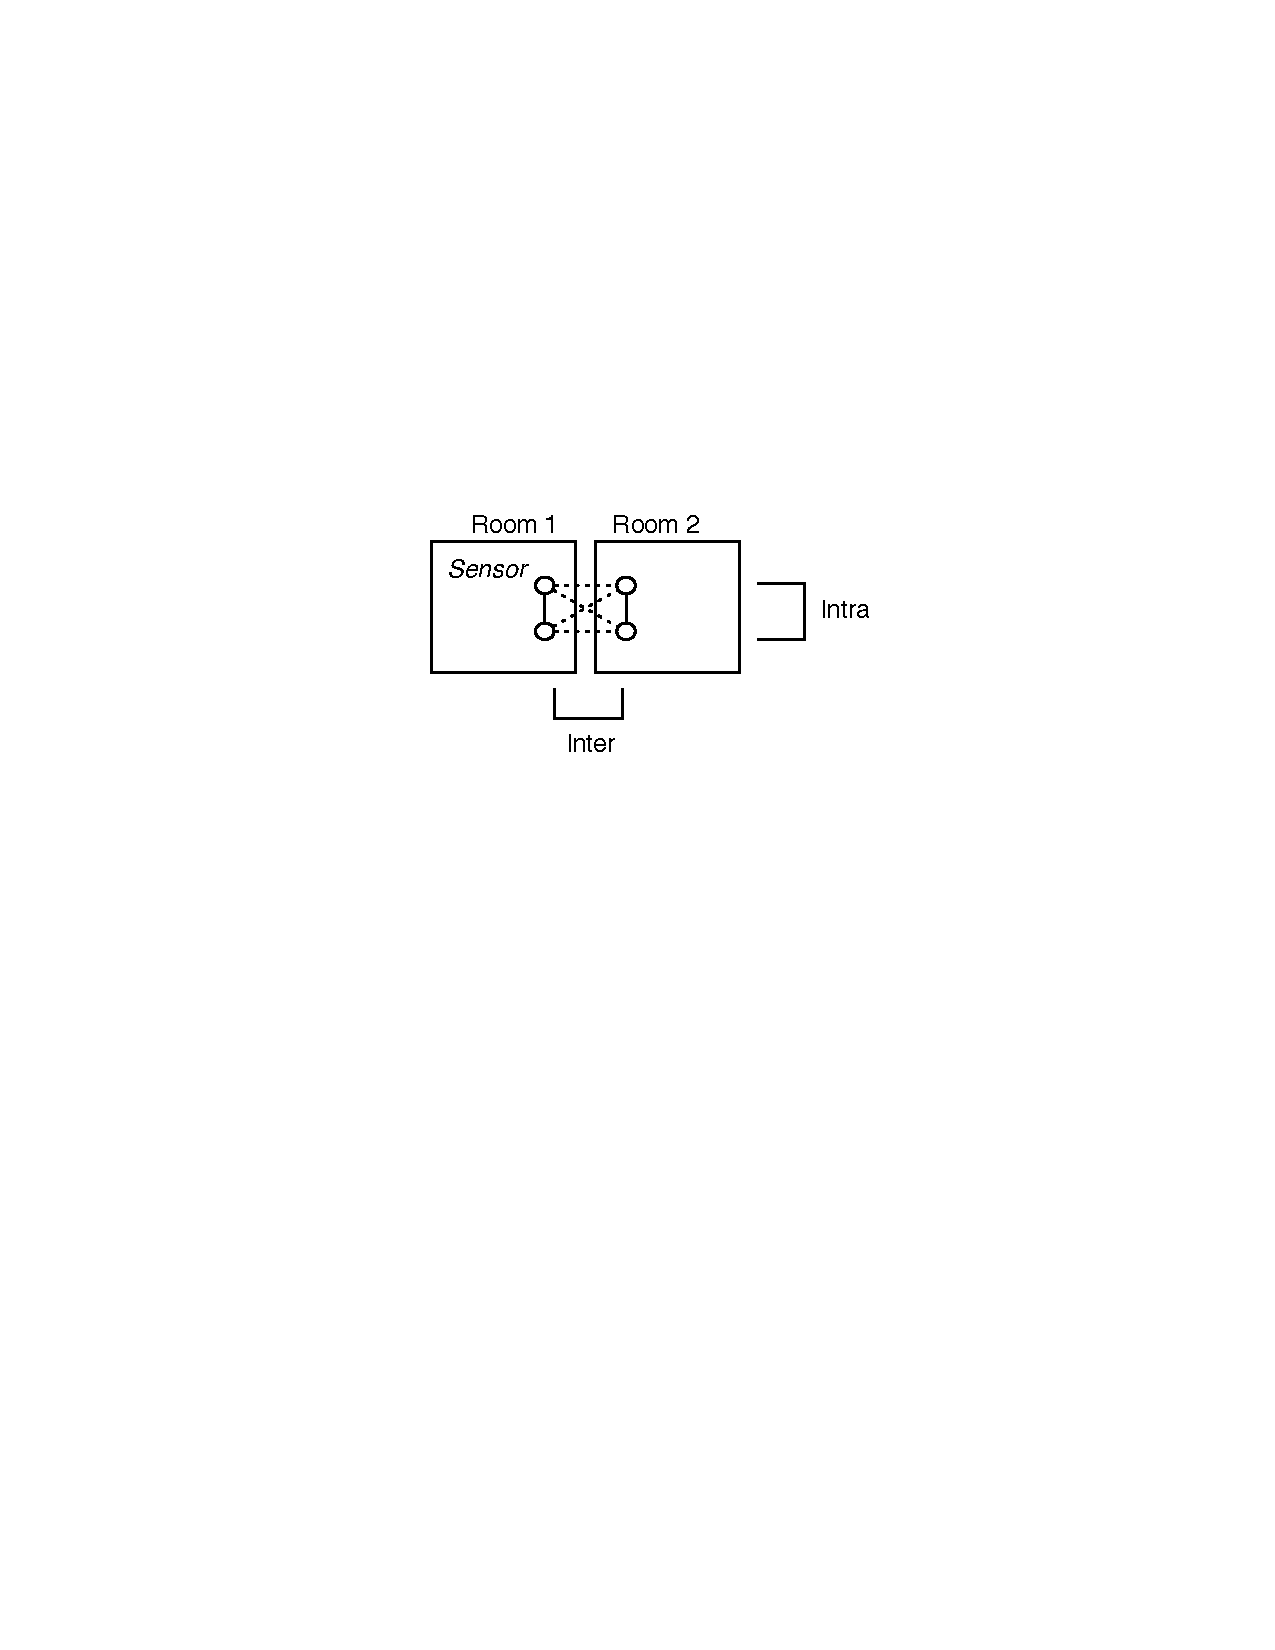
\includegraphics[width=0.65\textwidth]{figs/Inter_intra_relationships}
\caption{Two populations are examined for our threshold analysis.  A solid line connects sensors in the same room while a dotted line connects
 to a pairs in different rooms.}
\label{fig:group}
\end{figure}

\begin{figure}[h!]
\centering
	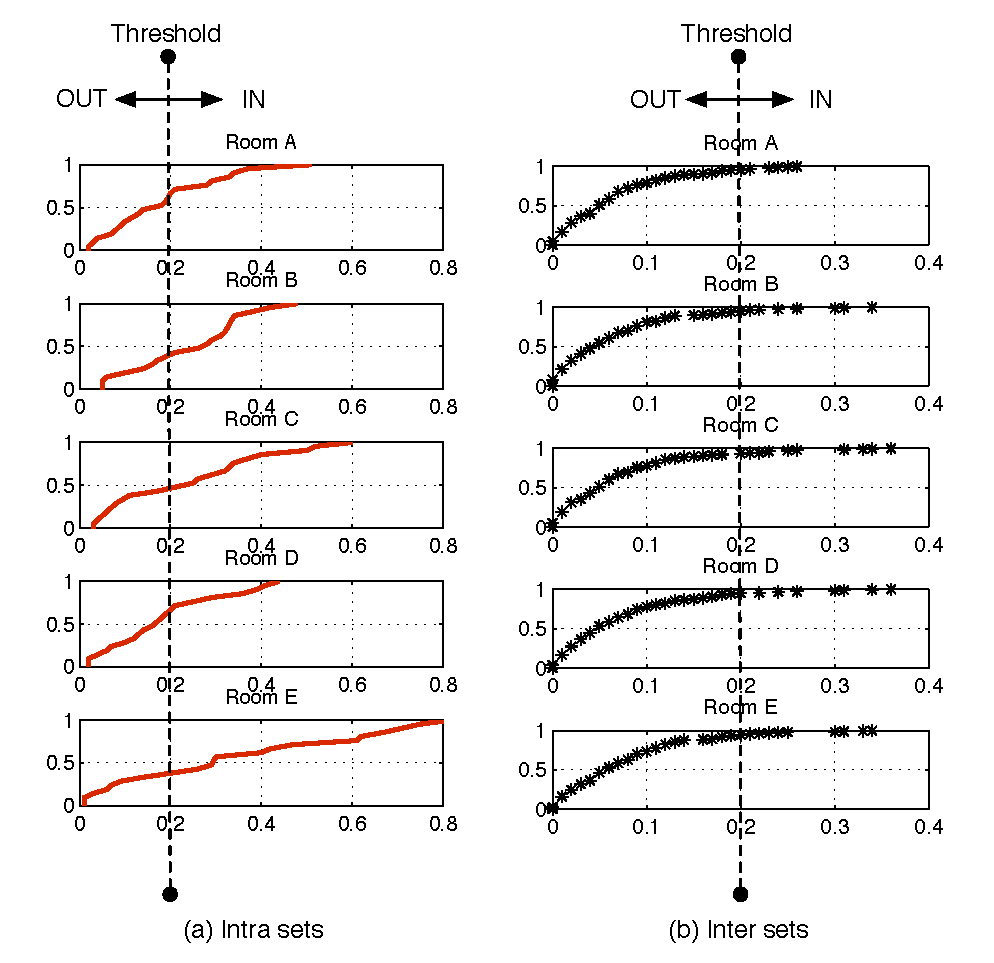
\includegraphics[width=1.0\textwidth]{figs/corrcoeff_cdf_in_out}
\caption{CDF of correlation coefficients between IMFs of sensor feeds: the dotted lines point to some threshold which divides
 the distribution and produces a TPR and FPR.
}
\label{fig:cdf}
\end{figure}

\subsubsection{Characterizing the Boundary}
To corroborate our boundary-existence hypothesis, we first need to characterize the boundary between sensors in different rooms. 
We compute the pairwise correlation coefficients (corrcoeffs) between sensor traces in both of populations depicted in Figure~\ref{fig:group}, 
over different time spans -- ranging from one day to one month.
After generating points over different time 
spans for each room, we accumulate the corrcoeffs to obtain distributions as shown in Figure~\ref{fig:cdf}, for each of the five rooms. 

The dashed vertical lines in Figure~\ref{fig:cdf} 
represent an arbitrary threshold that partitions the distribution into two sets.  Pairs of sensors to the right of the line
are classified as being in the same room.  Pairs of sensors to the left are classified as being in different rooms.
The CDFs on the left column show the distribution of corrcoeffs for pairs known to be in the same room and the CDFs on the right
show the distribution of corrcoeffs in different rooms.
Note in the figure, we set the threshold to the same value to both the left and right side, in order to observe the effect of the true/false positive
rates.
By adjusting the threshold, we get different TPRs/FPRs parameterized by the threshold. Figure~\ref{fig:roc} captures the range tradeoff in a corresponding ROC curve.


Figure~\ref{fig:roc} illustrates the TPR/FPR sensitivity to different threshold values for our method and the naive approach. A good cluster achieves a high TPR and a low FPR. 
As we vary the threshold, we see that our approach 
achieves a TPR between 52\%--93\% and a FPR between 5\%--59\%.  %The baseline, mostly remains along the diagonal, meaning it is practically random. 
We can see that the average TPR for the ROC graph on the right is higher than the 
ROC graph on the left.  Moreover, the corresponding average FPR is lower on the right than on the left.
In general, as the TPR rises, the FPR also goes up -- \emph{a tradeoff exists between maximizing TPR and maintaining a lower FPR}.


 The ``boundary'' is represented as the corrcoeff that produces a ``good" TPR with an ``acceptable" FPR.  In Figure~\ref{fig:rocA}, 
  we choose 0.2 FPR as the boundary threshold.  This point represents the largest difference between TPR and FPR -- an acceptable tradeoff point. 
Looking at Figure~\ref{fig:cdf}, the 0.2 FPR corresponds roughly to the 80th-percentile correlation coefficient, on the ``inter''
set (the set of CDFs on the right).
  The recall rate for each room -- using a 80th-percentile corrcoeff threshold value -- ranges between 62\%-86\% and the 
  threshold value falls into a narrow interval between 0.1 to 0.12. This shows that \emph{we are able to choose a uniform value 
  for all the rooms regardless of the sensor type.}

\subsection{Convergence over Time}
\begin{figure}[h!]
\centering
	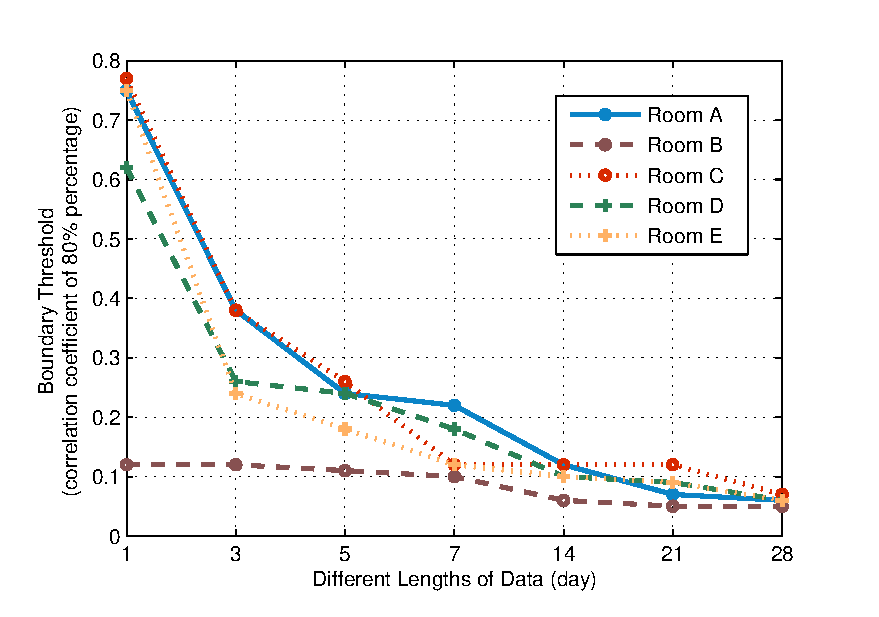
\includegraphics[width=0.48\textwidth]{figs/lengtheffect.eps}
\caption{The threshold values all converge to a similar value and we can derive the optimal value with as minimal as 14 days data.}
\label{fig:leneff}
\end{figure}

Using the threshold the roughly 80th-percentile corrcoeff corresponds to in the distribution, we examine how it affects the classification rate across traces
that span different lengths of time.  Convergence and consistency across different time spans is critical to automate the parameter selection
process.
Observe how the  threshold values differ quite significantly in Figure~\ref{fig:leneff}.  However, 
the threshold values 
gradually converge, as the length of training data increases from one day to one month.  The values derived after 14 days of data
are approximately the same as the final convergence value (around 0.07).  In other words, we can determine a threshold from two weeks of data.


\subsubsection{Clustering Results}
We cluster the sensor traces over the entire one-month period, and use the roughly 80th percentile corrceff (0.07) as the boundary threshold. 
A sensor is classified into the cluster with the largest corrcoeff. The clustering result is shown in Table~\ref{tab:cluster}.  A ``1" means the sensor is classified as inside the corresponding room. 
In general, after obtaining the sensor clusters, we don't know which room each cluster corresponds to without further information such as the metadata of sensors. The labels ``A-E" in Table~\ref{tab:cluster} are used to indicate the ground truth of where each sensor is physically placed since we have such information. Overall, the classification accuracy 
is 93.3\%.  We do not cluster on the corrcoeffs obtained among raw signals because the 80\%-percentile corrcoeff values do not converge across rooms.
The reason that we are able to get such a high accuracy, which is seemingly different from the statistics in Figure~\ref{fig:cdf} and Figure~\ref{fig:roc}, is because the statistics in the two figures are generated out of the corrcoeffs accumulated over different time spans (the same intervals in Figure~\ref{fig:leneff}) while the clustering here is performed on the corrcoeffs from the entire one-month period. 
% vary a lot and it doesn't make much sense to use different threshold for each room individually.

\begin{table}[h!]\footnotesize
 \begin{center}
	\begin{tabular}{ r|c|c|c|c|c|c }
	\multicolumn{1}{r}{}
	 &  \multicolumn{1}{c}{$A$}
	 & \multicolumn{1}{c}{$B$}
	 & \multicolumn{1}{c}{$C$}
	 & \multicolumn{1}{c}{$D$}
	  & \multicolumn{1}{c}{$E$} \\
	\cline{2-6} 
	$SensorA_{1}$ & 1 & 0 & 0 & 0 & 0 & \checkmark\\
	\cline{2-6}
	$A_{2}$ & 1 & 0 & 0 & 0 & 0 & \checkmark\\
	\cline{2-6}
	$A_{3}$ & 1 & 0 & 0 & 0 & 0 & \checkmark\\
	\cline{2-6}
	$B_{1}$ & 0 & 1 & 0 & 0 & 0 & \checkmark\\
	\cline{2-6}
	$B_{2}$ & 0 & 1 & 0 & 0 & 0 & \checkmark\\
	\cline{2-6}
	$B_{3}$ & 0 & 1 & 0 & 0 & 0 & \checkmark\\
	\cline{2-6}
	$C_{1}$ & 0 & 0 & 1 & 0 & 0 & \checkmark\\
	\cline{2-6}
	$C_{2}$ & 0 & 0 & 1 & 0 & 0 & \checkmark\\
	\cline{2-6}
	$C_{3}$ & 0 & 0 & 1 & 0 & 0 & \checkmark\\
	\cline{2-6}
	$D_{1}$ & 0 & 0 & 0 & 1 & 0 & \checkmark\\
	\cline{2-6}
	$D_{2}$ & 0 & 0 & 0 & 1 & 0 & \checkmark\\
	\cline{2-6}
	$D_{3}$ & 0 & 0 & 1 & 0 & 0 & $\times$\\
	\cline{2-6}
	$E_{1}$ & 0 & 0 & 0 & 0 & 1 & \checkmark\\
	\cline{2-6}
	$E_{2}$ & 0 & 0 & 0 & 0 & 1 & \checkmark\\
	\cline{2-6}
	$E_{3}$ & 0 & 0 & 0 & 0 & 1 & \checkmark\\
	\cline{2-6}
	\end{tabular}
 \end{center}
 \caption{Clustering result using the thresholding method: a ``1" means the sensor is classified as inside the room. We get the ``\checkmark" and ``$\times$" by comparing the clustering results with ground truth.}
 \label{tab:cluster}
\end{table}

\begin{figure*}[ht!]
\centering
	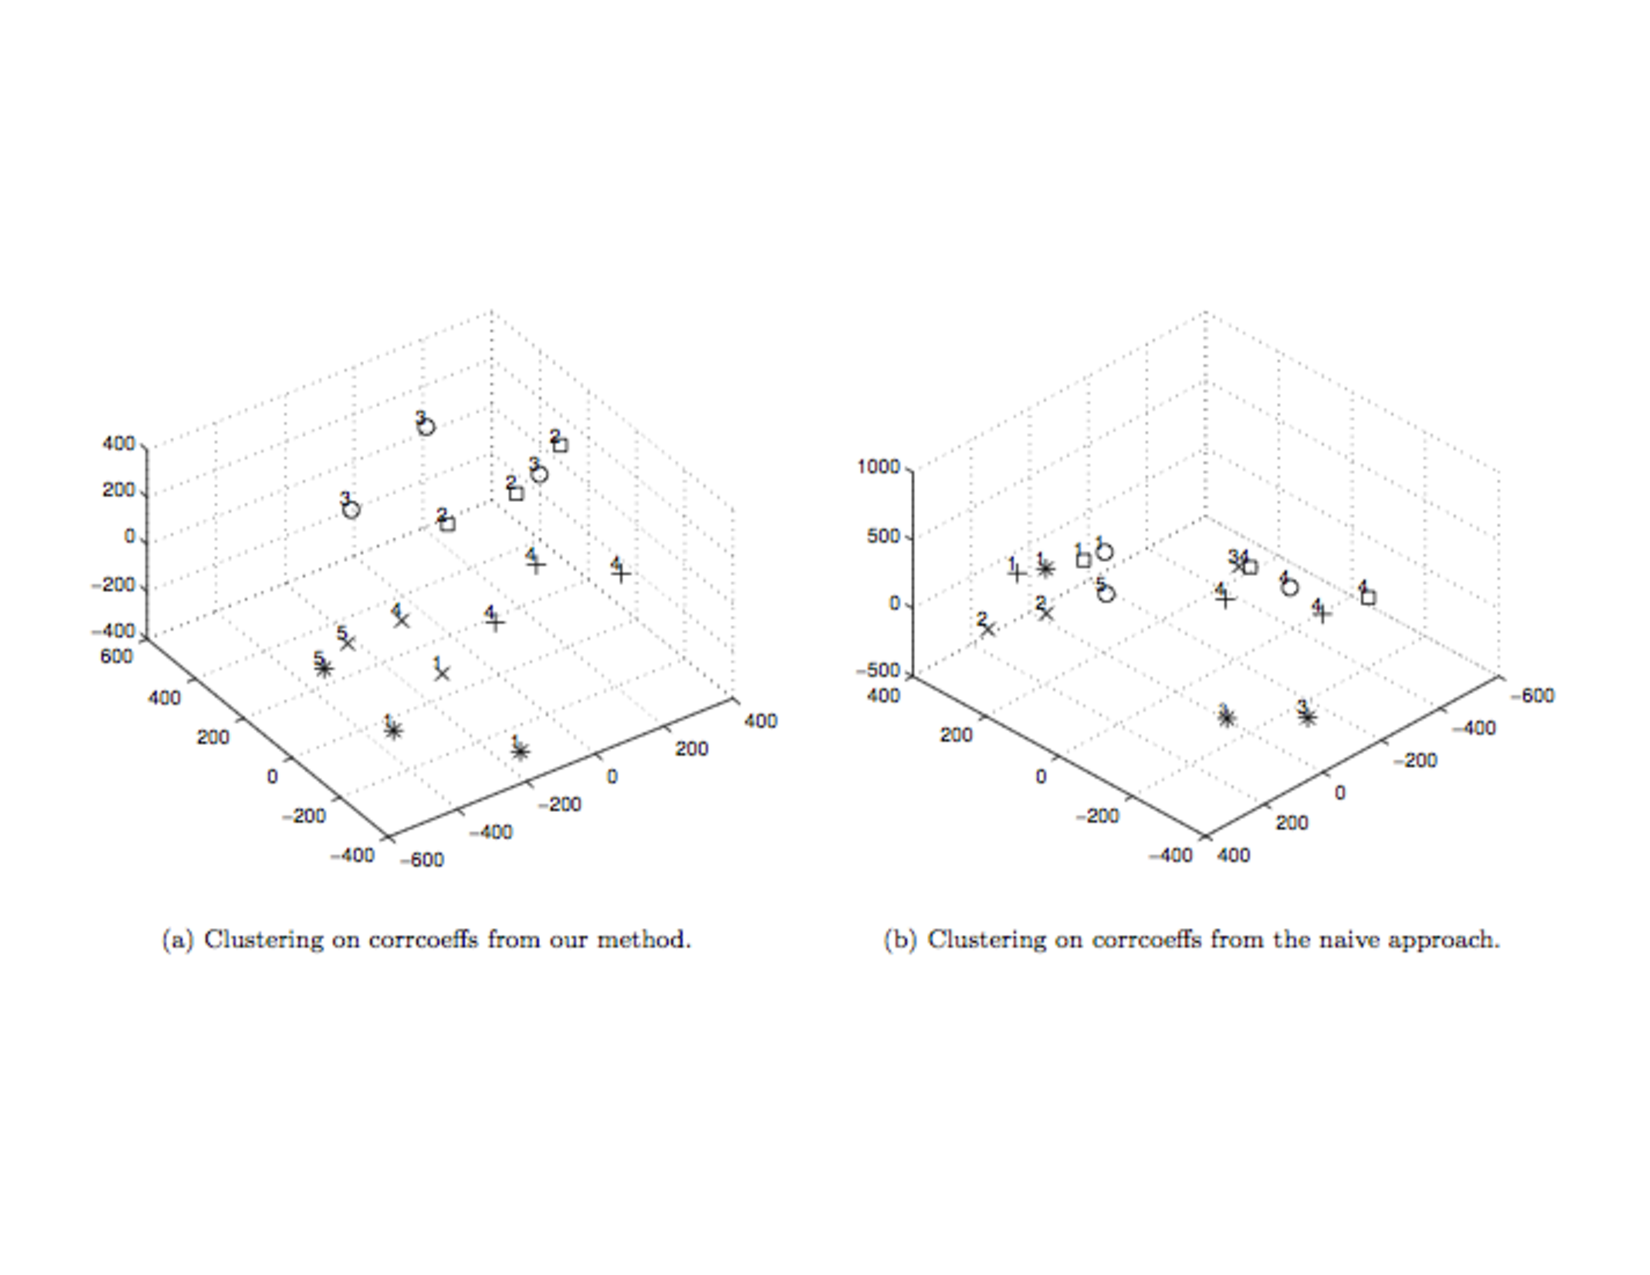
\includegraphics[width=1.0\textwidth]{figs/Space_KmeanClustering}
\caption{Clustering with k-means on the corrcoeff matrix after applying multidimensional scaling (MDS): The EMD-based set achieves an accuracy of 80\% while the results with raw-trace is only 53.3\% classification accuracy.}
\label{fig:mds}
\end{figure*}

To compare with our threshold-based method, we also cluster using a baseline approach. The pairwise corrcoeff for sensors in different rooms can be interpreted as a ``distance" between them.
A larger coefficient indicates a closer ``distance", and vice versa.  However, since the distances between pairs is relative, we use
multidimensional scaling~\cite{MDS} to find a common basis in three dimensions, re-map the relative distance metric (feature vector) into 
this three-dimensional grid and use k-means to classify the traces. % assuming the value of k is known a priori, which is the number of rooms.
We set k to equal the number of rooms, since the goal of the approach is to verify spatial placement at room-level granularity.  Generally, 
we believe that k should equal the number of rooms you wish to classify the sensors into. 
The clustering results are shown in Figure~\ref{fig:mds}.  Ground truth is shown through different markers (x, o, +, star, box). Each marker stands for one room. 
The cluster each sensor assigned to is denoted with a number. The classification accuracy of the baseline approach on corrcoeffs matrix of re-aggregated IMFs is 80\%. 
For raw traces, the baseline approach achieves an accuracy of only 53.3\%.






